\section{Introdução}

Nas eleições brasileiras de 2022, houve um grande movimento conhecido como Passe Livre pela Democracia, que lutou pela adoção do transporte público gratuito no dia da votação, para que mais pessoas votassem. O movimento enfrentou bastante resistência política e foi grande alvo de discussão. 

Essa medida tem seu mérito divido em dois aspectos, o primeiro deles sendo normativo, considerando a mobilidade como um direito e a dificuldade de uma pessoa se locomover à urna como uma possível barreira monetária ao exercício democrático de votar. O segundo aspecto se refere aos incentivos econômicos do voto, sendo que um estímulo monetário influencia a decisão das pessoas e pode ser decisivo para ``convencer'' um cidadão a votar.

Entretanto, esta medida pode ser um tanto quanto custosa e não há garantias de que as pessoas que usufruem do passe livre efetivamente estão aproveitando a medida para votar ou para realizar outras atividades. \textcite{pereira2023transporte} conduzem um estudo na tentativa de identificar essa hipótese, e seus resultados serão discutidos no tópico \ref{subsec_revisao}. Ademais, o conturbado cenário político complicou a execução da medida, visto que a comunicação dos governos municipais pode não ter sido eficiente e possivelmente a população não estava plenamente ciente da adoção do passe livre. 

O objetivo deste estudo é identificar se a adoção do passe livre causa uma redução na abstenção. Na seção \ref{sec_teor} é discutido o que é estabelecido na teoria de ciência política com um olhar microeconômico, bem como é feita uma adaptação dos modelos da literatura para o caso do passe livre. Na seção \ref{sec_modEmp} é feita uma tentativa empírica de medir o efeito do passe livre a partir de um \textit{diff-in-diff} pareado com efeitos fixos e um \textit{event study} para testes de robustez.

\section{Modelagem Teórica}
\label{sec_teor}

\subsection{Revisão Literária}
\label{subsec_revisLit}

A discussão sobre abstenção é extensiva no campo da economia política e diversos autores contribuíram com o debate de seus determinantes. \textcite{downs1957economic} é um dos precursores do modelo microeconômico que é continuado por uma série de autores. Sua premissa é simples: os eleitores buscam maximizar suas utilidades, que são definidas pela Equação \ref{eq_downs}. A partir disso, é considerado racional o eleitor que vota quando sua utilidade esperada é maior que zero e, caso contrário, se abstém. 

\begin{equation}
\label{eq_downs}
    \mathbb{E}(U_i)=B\cdot P-C
\end{equation}

Na equação, $\mathbb{E}(U_i)$ representa a utilidade esperada do cidadão $i$ apto, ao votar. Esta utilidade é impactada negativamente por $C$, o custo de votar, que se refere aos dispêndios de tempo, recursos e custos de oportunidade. Exemplos de fatores que podem afetar o custo são longas distâncias até as urnas, filas e demora para votar, o custo financeiro do transporte, fortes chuvas, etc. Os custos de não votar, como a necessidade de justificar o voto e pagar uma multa no caso brasileiro, são considerados nesse custo também afetando positivamente a utilidade de votar. A variável $B$ representa o benefício líquido de seu candidato favorito, caso seja eleito. Na análise de Downs, o benefício é dado por quanto o eleitor julga que sua primeira opção de candidato (A) seja melhor que a segunda opção (B), caso seja eleita: $B_{it} = \mathbb{E}(U^A_{t+1})-\mathbb{E}(U^B_{t+1})$. $P$ representa a probabilidade de seu voto ser decisivo. O voto decisivo é considerado aquele que desempata o resultado da eleição, caso o número de votantes seja ímpar, ou defina o resultado da votação, caso seja par. Em termos práticos, o benefício do candidato preferido apenas será importante para o eleitor, caso o seu voto seja a causa dele ser eleito.

O modelo apresenta uma série de complicações, que são inclusive discutidas de forma descritiva por Downs. Um eleitor indiferente entre os candidatos neste modelo apresenta benefício zero e não votaria para qualquer valor de $C$ positivo, então não seria racional votar branco. Além disso, em eleições de grande escala, como é o caso das eleições federais que apresentam mais de 150 milhões de votantes, a probabilidade do voto ser decisivo é muito próxima a zero. Nesses casos, caso o custo seja positivo, a utilidade do voto seria sempre negativa e ninguém votaria.

Para endereçar estes problemas, \textcite{riker1968theory} introduzem, entre outras contribuições, mais um componente autônomo da utilidade
\footnote{É considerado um componente autônomo aquele que não está relacionado à abstenção. Considerando que a probabilidade do voto ser decisivo é dada por $P = 1/v$, no qual v é o número de votantes, quanto maior for a abstenção, maior é a probabilidade do voto ser decisivo}
$D$. Este se refere ao dever cívico de votar, que não está relacionado à probabilidade do voto ser decisivo. O autor argumenta que há um ganho de utilidade ao contribuir com o sistema democrático, bem como pode haver o sentimento de arrependimento caso o sujeito se abstenha. Além disso, considera votar um ato político, relacionado à tradição. Por outro lado, reconhece que para a maior parte das pessoas $D<C$ e, portanto, ainda não seria racional votar em grandes eleições.

\begin{equation}
\label{eq_riker}
    \mathbb{E}(U_i)=B\cdot P-C+D
\end{equation}

Os pesquisadores da escolha racional geralmente são muito focados no interesse individual das escolhas, mas no final do século XX uma série de estudos e experimentos passaram a questionar e contribuir com evidências de comportamentos racionalmente altruístas. Alguns modelos de escolha racional foram revisitados e \textcite{fowler2006altruism} e \textcite{edlin2007voting} são autores que incorporam este componente no modelo de forma a dividir o benefício líquido em duas partes (Equação \ref{eq_fowler}). A variável $B_p$ se refere ao benefício líquido que o candidato proporciona ao indivíduo, enquanto $B_s$ se refere ao benefício social. A questão é que enquanto $B_p$ beneficia apenas o sujeito, $B_s$ beneficia a todos no país na visão do eleitor, então este benefício é multiplicado pela população $N$. Entretanto, o benefício social não necessariamente apresenta a mesma relevância ao eleitor, se comparado ao individual e $\alpha$ controla por este fator, de forma que para a maioria das pessoas $0<\alpha < 1$.

\begin{equation}
\label{eq_fowler}
    B_i = B_p + \alpha\cdot NB_s
\end{equation}

Outra contribuição de \textcite{edlin2007voting} foi de consolidar o que se considera a probabilidade do voto ser decisivo (Equação \ref{e1_edlin}). O coeficiente $K$ representa o grau de competitividade da eleição e quanto mais próximas forem os votos do candidato A em relação ao B, maior é a probabilidade do voto ser decisivo. Em uma votação em que a diferença de votos entre os candidatos está em torno de $10p.p$., $K=5$, enquanto uma diferença de $\pm 2p.p.$ resulta em um $K=25$. Portanto, a probabilidade do voto ser decisivo $P$ é dada pela competitividade dividida pelo número de votantes, que equivale ao total de eleitores elegíveis $E$ vezes taxa de comparecimento $t$.

\begin{equation}
\label{e1_edlin}
\begin{aligned}
    K &= \frac{1}{\log(V_A)-\log(V_B)}\\
    P &= K/(tE)
\end{aligned}
\end{equation}

Ao substituir as equações \ref{eq_fowler} e \ref{e1_edlin} em \ref{eq_riker}, têm-se a equação em sua forma final (Equação \ref{eq_final}). É interessante observar que na medida em que o número de votantes $V$ aumenta, o benefício pessoal se aproxima a zero, enquanto o benefício social não, pois quando o número de votantes aumenta, o número de pessoas beneficiadas $N$ também aumenta. Considerando os fatores agregados, as ideias primordiais de \textcite{downs1957economic} tornam-se mais robustas, mas o esqueleto se mantém igual: $\alpha NB_s$ representam o benefício líquido do voto, $\frac{K}{tE}$ é a probabilidade do voto ser decisivo e $C+D$ é o componente autônomo do voto.

\begin{equation}
\label{eq_final}
\begin{aligned}
    \mathbb{E}(U_i)&=(B_p + \alpha\cdot NB_s)\cdot \frac{K}{tE}-C+D\\
    &=\left(\cancel{\frac{B_p}{V}} + \frac{\alpha\cdot NB_s}{tE}\right)\cdot K-C+D\\
    &=\underbrace{\frac{\alpha NB_s}{1}}_B\cdot\underbrace{\frac{K}{tE}}_P-\underbrace{C+D}_A
\end{aligned}
\end{equation}

Um desdobramento peculiar desse modelo é uma espécie de paradoxo, que inclusive foi discutido por \textcite{downs1957economic}. Nessa relação paradoxal, quanto maior é a utilidade de votar $\uparrow\mathbb{E}(U_i)$, mais pessoas votam $\uparrow t$, o que diminui a utilidade de votar $\downarrow\mathbb{E}(U_i)$, reduzindo o número de pessoas que votam $\downarrow t$. Em outras palavras, a relação entre a utilidade de voto e comparecimento é um ciclo de balanceamento. Quando uma variável exógena, como o custo, altera a utilidade do voto, há um efeito multiplicador que atenua a mudança no comparecimento. 

\begin{figure}
    \centering
    % \begin{tikzpicture}[
%     node distance=12mm,
%     >=stealth, auto,
% every state/.style={draw=none}
%                 ]
% \node[state] (q12)                  {$14$};
% \node[state] (q24) [below=of q12]   {$34$};
%     \begin{scope}[bend left]%
% \path[->]   (q12.south east) edge node {c} (q24.north east)
%             (q24.north west) edge node {c} (q12.south west);
%     \end{scope}
% \end{tikzpicture}

\begin{tikzpicture}[
    node distance=30mm, % Increase the distance to accommodate horizontal positioning
    >=stealth, auto,
    every state/.style={draw=none}
]
    \node[state] (q12)                  {$\mathbb{E}(U_i)$};
    \node[state] (q24) [right=of q12]   {$t$}; 
    \node[state] (q1) [left=of q12]     {$C$}; 

    \begin{scope}[bend left]%
        \path[->]   (q12.north east) edge node {$(+)$} (q24.north west) 
                    (q24.south west) edge node {$(-)$} (q12.south east)
                    (q1.east) edge node {$(-)$} (q12.west);

        \path ($(q12.east)!0.5!(q24.west)$) node[circle, draw] (B) {B};
        
    \end{scope}
\end{tikzpicture}
    \caption{Paradoxo de Downs: ciclo de balanceamento.}
    \label{cycle}
\end{figure}

\subsection{Extensão do modelo e resultados teóricos}

A partir do modelo apresentado é possível intuir o que aconteceria a nível agregado dada uma mudança em alguma das variáveis. Para tanto, é necessário estabelecer um sistema que determine a abstenção de equilíbrio -- a partir dele será possível analisar como o equilíbrio é deslocado. O equilíbrio de comparecimento $t_{eq}$ é dado quando todos os cidadãos elegíveis escolhem de forma a maximizarem suas utilidades, ou seja, aqueles que apresentam utilidade esperada maior que zero votam, caso contrário, se abstêm. Esse ponto se encontra na intersecção entre a função de benefício marginal do voto e custo marginal do voto (Equação \ref{eq_static}). 

Na figura \ref{fig_static1} é possível observar para qualquer nível de comparecimento $t$ menor do que o comparecimento de equilíbrio $t_{eq}$, haveria eleitores que apresentariam utilidade esperada positiva de votar, o que torna a ação de votar uma escolha racional e, portanto, mais pessoas votariam deslocando o comparecimento ao equilíbrio. De maneira semelhante, caso fosse observado um comparecimento acima do equilíbrio, eleitores apresentam utilidade esperada de votar negativa, sendo racional que se abstenham. Com este modelo, é possível identificar de que forma o equilíbrio se desloca, dada uma variação em alguma das variáveis.

\begin{equation}
\label{eq_static}
\begin{aligned}
    C_{mg}&= B_{mg}\\
    C &=\left(\frac{\alpha\cdot B_s\cdot N\cdot K}{E\cdot t_{eq}^e}\right)+D \\
    t_{eq}^e&=\left(\frac{\alpha\cdot B_s\cdot N\cdot K}{E\cdot (C-D)}\right)
\end{aligned}
\end{equation}

\begin{figure}[!ht]
    \begin{subfigure}[t]{0.45\linewidth}
      \begin{tikzpicture}
\begin{axis}[standard,
    xtick={0.2, 0.4, 0.6, 0.8, 1},
    ytick={\varC,\varD},
    yticklabels = {$C$, $D$},
    samples=\nsamples,
    ylabel near ticks,
    xlabel near ticks,
    xlabel={Comparecimento $t$},
    ylabel={$C_{mg},B_{mg}$},
    xmin=0,xmax=1,
    ymin=0,ymax=4
]

% \node[anchor=center] at (axis cs:0,0){};
\draw[dashed] (0,\varD)--(1,\varD);
\draw[] (1,0)--(1,10);

\addplot[name path=F,domain={0:1}]{\varA/x + \varD};
\addplot[name path=G,domain={0:1}]{\varC};

\addplot[fill=blue, fill opacity=0.2] fill between [of=F and G, soft clip={domain=0 : 0.4/0.7}];
\addplot[fill=red, fill opacity=0.2] fill between [of=F and G, soft clip={domain=0.4/0.7 : 1}];
\path [name intersections={of=G and F}]; 
\coordinate [label= $t_{eq}$ ] (OP1) at (intersection-1);
\fill [black] (OP1) circle (1pt);

\end{axis}
\end{tikzpicture}



      \caption{Oferta e demanda de votos}
      \label{fig_static1}
    \end{subfigure}
    \hfill
    \begin{subfigure}[t]{0.45\linewidth}
      \begin{tikzpicture}
\begin{axis}[standard,
    xtick={1.5,1.8,2.5,2.8},
    ytick={1},
    yticklabels = {1},
    xticklabels = {$C_{A_{1}}$, $C_{A_{0}}$, $C_{B_{1}}$, $C_{B_{0}}$},
    samples=\nsamples,
    xlabel={$C$},
    ylabel={$\frac{\partial{(t_{eq}})}{\partial C}$},
    xmin=1.2,xmax=3,
    ymin=-1,ymax=0.1,
    tick label style={above, font=\tiny}
]

\addplot[name path=F,domain={0.6:10}]{-\varA/((x - \varD)^2)};
\addplot[name path=G,domain={0.6:10}]{0};

\addplot[fill=black, fill opacity=0.2] fill between [of=F and G, soft clip={domain= 1.5 : 1.8}];
\addplot[fill=black, fill opacity=0.2] fill between [of=F and G, soft clip={domain= 2.5 : 2.8}];

\draw[dotted] (1.5,0)--(1.5,-1.2);
\draw[dotted] (1.8,0)--(1.8,-1.2);
\draw[dotted] (2.5,0)--(2.5,-1.2);
\draw[dotted] (2.8,0)--(2.8,-1.2);

\draw [decorate, 
    decoration = {
        calligraphic brace,
        raise = 10pt
    }
] (1.5,0) --  (1.8,0) node[pos=0.5,above=10pt,black]{$\Delta C_A$};

\draw [decorate, 
    decoration = {
        calligraphic brace,
        raise = 10pt
    }
] (2.5,0) --  (2.8,0) node[pos=0.5,above=10pt,black]{$\Delta C_B$};


\end{axis}
\end{tikzpicture}
      \caption{Derivada parcial do comparecimento de equilíbrio em relação ao custo}
      \label{fig_static2}
    \end{subfigure}
    \caption{Visualização do modelo microeconômico}
    \label{fig_staticA}
  \end{figure}

% \begin{minipage}{0.3\linewidth}
% \begin{tikzpicture}
\begin{axis}[standard,
    xtick={0.2, 0.4, 0.6, 0.8, 1},
    ytick={\varC,\varD},
    yticklabels = {$C$, $D$},
    samples=\nsamples,
    ylabel near ticks,
    xlabel near ticks,
    xlabel={Comparecimento $t$},
    ylabel={$C_{mg},B_{mg}$},
    xmin=0,xmax=1,
    ymin=0,ymax=4
]

% \node[anchor=center] at (axis cs:0,0){};
\draw[dashed] (0,\varD)--(1,\varD);
\draw[] (1,0)--(1,10);

\addplot[name path=F,domain={0:1}]{\varA/x + \varD};
\addplot[name path=G,domain={0:1}]{\varC};

\addplot[fill=blue, fill opacity=0.2] fill between [of=F and G, soft clip={domain=0 : 0.4/0.7}];
\addplot[fill=red, fill opacity=0.2] fill between [of=F and G, soft clip={domain=0.4/0.7 : 1}];
\path [name intersections={of=G and F}]; 
\coordinate [label= $t_{eq}$ ] (OP1) at (intersection-1);
\fill [black] (OP1) circle (1pt);

\end{axis}
\end{tikzpicture}



% \end{minipage}
% \hspace{0.1\linewidth}   
% \begin{minipage}{0.3\linewidth}
% \begin{tikzpicture}
\begin{axis}[standard,
    xtick={1.5,1.8,2.5,2.8},
    ytick={1},
    yticklabels = {1},
    xticklabels = {$C_{A_{1}}$, $C_{A_{0}}$, $C_{B_{1}}$, $C_{B_{0}}$},
    samples=\nsamples,
    xlabel={$C$},
    ylabel={$\frac{\partial{(t_{eq}})}{\partial C}$},
    xmin=1.2,xmax=3,
    ymin=-1,ymax=0.1,
    tick label style={above, font=\tiny}
]

\addplot[name path=F,domain={0.6:10}]{-\varA/((x - \varD)^2)};
\addplot[name path=G,domain={0.6:10}]{0};

\addplot[fill=black, fill opacity=0.2] fill between [of=F and G, soft clip={domain= 1.5 : 1.8}];
\addplot[fill=black, fill opacity=0.2] fill between [of=F and G, soft clip={domain= 2.5 : 2.8}];

\draw[dotted] (1.5,0)--(1.5,-1.2);
\draw[dotted] (1.8,0)--(1.8,-1.2);
\draw[dotted] (2.5,0)--(2.5,-1.2);
\draw[dotted] (2.8,0)--(2.8,-1.2);

\draw [decorate, 
    decoration = {
        calligraphic brace,
        raise = 10pt
    }
] (1.5,0) --  (1.8,0) node[pos=0.5,above=10pt,black]{$\Delta C_A$};

\draw [decorate, 
    decoration = {
        calligraphic brace,
        raise = 10pt
    }
] (2.5,0) --  (2.8,0) node[pos=0.5,above=10pt,black]{$\Delta C_B$};


\end{axis}
\end{tikzpicture}
% \end{minipage}

\begin{equation}
\label{eq_parcial}
    \frac{\partial{(t_{eq}^e})}{\partial C} = -\left(\frac{\alpha\cdot B_s\cdot N\cdot K}{E\cdot (C-D)^2}\right)
\end{equation}

A equação \ref{eq_parcial} apresenta a derivada parcial do equilíbrio de comparecimento em relação ao custo do voto. Na medida em que o custo aumenta, \textit{ceteris paribus}, o comparecimento reduz. Na figura \ref{fig_static2} é possível observar qual é o impacto de um $\Delta C$ no comparecimento, visto que a área pintada abaixo do gráfico representa a quantidade de pessoas que foram "convencidas"\  a votar por conta da redução do custo e, caso houvesse um aumento, representaria a quantidade de pessoas que desistiram de votar. Um ponto importante é que um $\Delta C$ impacta de maneira heterogênea localidades com níveis de comparecimento diferentes: em municípios cujo comparecimento é baixo, um $\Delta C$ surte efeito diminuto, enquanto em um município com comparecimento alto, um $\Delta C$ pequeno pode causar diferenças significativas. Isso ocorre, pois a função de benefício marginal é recíproca
\footnote{A função do benefício marginal $(B_{mg}=\frac{Z}{t_{eq}} + D)$, na qual $Z$ representa todas as variáveis que multiplicam $t_{eq}$ é recíproca, já que depende inversamente do comparecimento de equilíbrio} 
e assintótica em $D$, ou seja, na medida em que o comparecimento aumenta, o benefício marginal se aproxima de $D$, o dever cívico do voto. Nesse sentido, quando o comparecimento é muito alto, o principal fator que define o equilíbrio é a diferença entre $C$ e $D$.

Entretanto, um fator que não pode ser ignorado é de que estas variáveis todas se referem às expectativas das pessoas. A competitividade da eleição, por exemplo, é dada pela percepção dos eleitores com base nas pesquisas eleitorais, conteúdo da mídia e interações com seus conhecidos. Nesse sentido, o comparecimento de equilíbrio é dado por expectativas prévias à eleição, que não necessariamente se confirmam no dia da votação. Na equação \ref{eq_expectativas}, tem-se que o comparecimento esperado de equilíbrio é dado pelo verdadeiro equilíbrio $t_{eq}$, mais um erro de expectativas oriundo de assimetria de informações $\varepsilon$. Substituindo a equação \ref{eq_expectativas} em \ref{eq_static}, incorpora-se um componente de expectativas na estática comparativa.

\begin{equation}
\label{eq_expectativas}
    t_{eq}^{e} = t_{eq} + \varepsilon
\end{equation}

Este componente permite analisar o efeito que a assimetria de informações pode causar. Na figura \ref{fig_static3} é possível observar como o comparecimento de equilíbrio se desloca quando há uma redução no custo sem que haja assimetria de informações. Entretanto, na figura \ref{fig_static4}, é anunciada uma redução no custo para todos os eleitores, mas no dia da eleição esta redução não ocorre, sem que as pessoas fossem avisadas. Neste caso, há uma assimetria de informações e os eleitores antecipam um número maior de eleitores por causa da redução do custo, que reduz a utilidade de seus votos via menor probabilidade dele ser decisivo, criando desincentivos para o voto. Dessa forma, há um aumento em $\varepsilon$, que desloca a curva de benefício marginal para baixo e se observa o comparecimento na intersecção da curva de custo marginal, que efetivamente não se desloca, com a nova curva de benefício marginal. Este equilíbrio, inclusive, é de um comparecimento menor do que tinha se não fosse anunciada a redução no custo.

\begin{figure}[!ht]
    \begin{subfigure}[t]{0.45\linewidth}
      \begin{tikzpicture}
\begin{axis}[standard,
    xtick={0.2, 0.4, 0.6, 0.8, 1},
    ytick={\varC,\varD},
    yticklabels = {$C$, $D$},
    samples=\nsamples,
    ylabel near ticks,
    xlabel near ticks,
    xlabel={Comparecimento $t$},
    ylabel={$C_{mg},B_{mg}$},
    xmin=0,xmax=1,
    ymin=0,ymax=4
]

% \node[anchor=center] at (axis cs:0,0){};
\draw[dashed] (0,\varD)--(1,\varD);
\draw[] (1,0)--(1,10);

\addplot[name path=F,domain={0:1}]{\varA/x + \varD};
\addplot[name path=G,domain={0:1}, dotted]{\varC};
\addplot[name path=Gg,domain={0:1}]{\varC-0.13};


\path [name intersections={of=G and F}]; 
\coordinate [label= $t_{eq}$ ] (OP1) at (intersection-1);
\fill [black] (OP1) circle (1pt);

\path [name intersections={of=Gg and F}]; 
\coordinate (OP2) at (intersection-1);
\fill [black] (OP2) circle (1pt);
\node [below] at (OP2) {$t_{eq}'$};

\end{axis}
\end{tikzpicture}
      \caption{Sem assimetria de informações}
      \label{fig_static3}
    \end{subfigure}
    \hfill
    \begin{subfigure}[t]{0.45\linewidth}
      \begin{tikzpicture}
\begin{axis}[standard,
    xtick={0.2, 0.4, 0.6, 0.8, 1},
    ytick={\varC,\varD},
    yticklabels = {$C$, $D$},
    samples=\nsamples,
    ylabel near ticks,
    xlabel near ticks,
    xlabel={Comparecimento $t$},
    ylabel={$C_{mg},B_{mg}$},
    xmin=0,xmax=1,
    ymin=0,ymax=4
]

% \node[anchor=center] at (axis cs:0,0){};
\draw[dotted] (0,\varD)--(1,\varD);
\draw[] (1,0)--(1,10);

\addplot[name path=F,domain={0:1}, dashed]{\varA/x + \varD};
\addplot[name path=Ff,domain={0:1}]{(\varA - 0.1)/x + \varD};

\addplot[name path=G,domain={0:1}]{\varC};
\addplot[name path=Gg,domain={0:1}, dotted]{\varC-0.13};


\path [name intersections={of=G and F}]; 
\coordinate [label= $t_{eq}$ ] (OP1) at (intersection-1);
\fill [black] (OP1) circle (1pt);

\path [name intersections={of=Gg and F}]; 
\coordinate (OP2) at (intersection-1);
\fill [black] (OP2) circle (1pt);
\node [below] at (OP2) {$t_{eq}^e$};

\path [name intersections={of=G and Ff}]; 
\coordinate (OP3) at (intersection-1);
\fill [black] (OP3) circle (1pt);
\node [below] at (OP3) {$t_{obs}$};

\end{axis}
\end{tikzpicture}
      \caption{Com assimetria de informações}
      \label{fig_static4}
    \end{subfigure}
    \caption{Estática comparativa e \textit{moral hazard}}
    \label{fig_staticB}
  \end{figure}

Portanto, do ponto de vista teórico, uma medida de redução do custo de votar com a intenção de aumentar o comparecimento, por conta da assimetria de informações pode acabar por diminuí-lo. Esse fenômeno se configura como um \textit{moral hazard}. No caso do passe livre, um município pode cair nessa armadilha caso adote o passe livre, mas as pessoas não efetivamente utilizem o transporte público para votar ou a redução no custo não convença o número esperado de pessoas a votar. Apesar desse risco existir, ainda é possível que mesmo com assimetria de informações o comparecimento aumente, dependendo do grau da assimetria.  
  
\section{Modelagem Empírica}
\label{sec_modEmp}

\subsection{Revisão da literatura empírica}
\label{subsec_revisao}

Há apenas um estudo que analisa o impacto do passe livre adotado em 2022 na abstenção, conduzido por \cite{pereira2023transporte}. O estudo traz uma contribuição inovadora utilizando dados de celular para identificar padrões de mobilidade no dia da eleição, com base na localização do usuário. Segundo os autores:

\begin{quote}
    ``Não encontramos qualquer efeito da gratuidade no transporte público sobre
    o comparecimento às urnas ou sobre os resultados eleitorais, mas encontramos um efeito positivo,
    entre 7,2\% e 17,5\% de aumento, nos níveis de mobilidade no dia das eleições. Embora a redução
    dos custos monetários de transporte possa melhorar o acesso das pessoas aos locais de votação,
    nossos resultados sugerem que apenas políticas de redução desses custos não são suficientes
    para aumentar o comparecimento dos eleitores.'' 

    ``Assim, os governos podem justificar a adoção de políticas de isenção de tarifas por motivos normativos [...], mas sabendo que tais políticas podem não efetivamente trazer mais eleitores às urnas.''
\end{quote}

Entretanto, associada à forte afirmação sobre as políticas de redução de custos que vai na contramão da literatura teórica, há algumas pontos a serem levantados em relação à interpretação dos resultados. O primeiro comentário que deve ser feito se refere à afirmação sobre o aumento nos níveis de mobilidade. Os autores identificam que houve aumento de mobilidade nos municípios que adotaram o passe livre em relação aos que não adotaram -- efeito não encontrado para aumento do comparecimento --, mas a hipótese de identificação é bastante frágil nesta inferência. 

\begin{figure}[!ht]
    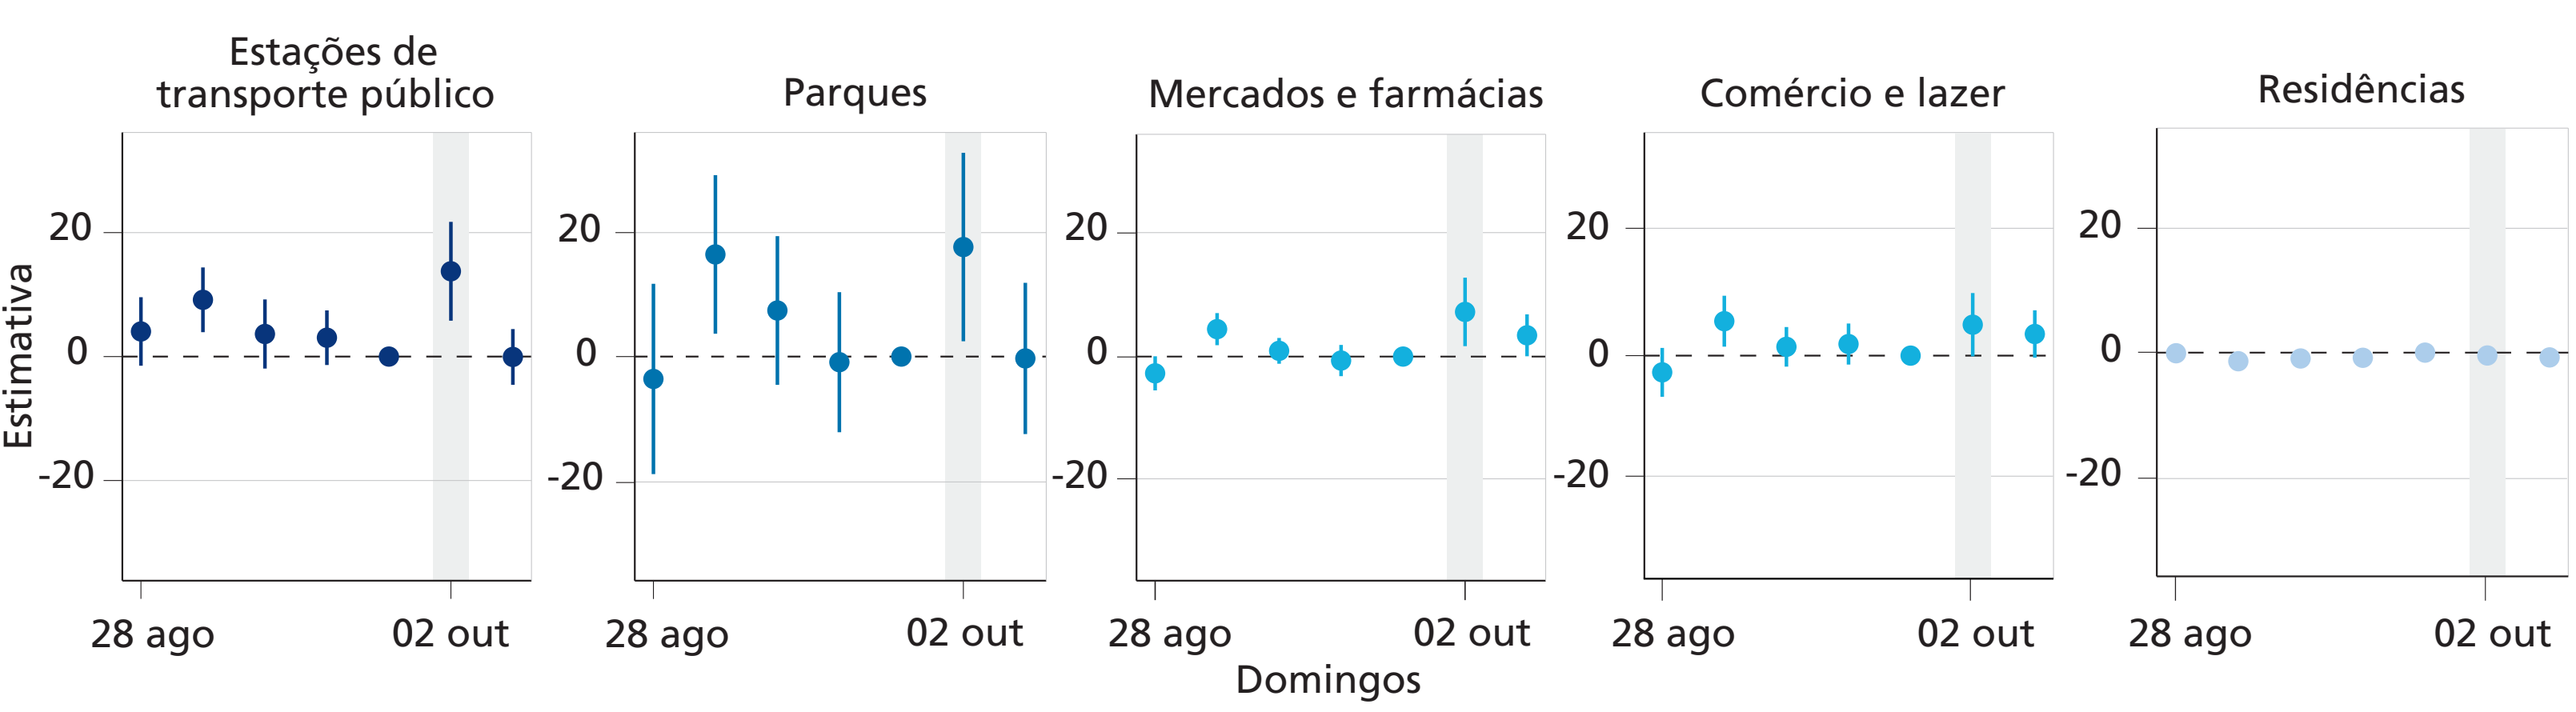
\includegraphics[width = \linewidth]{passe-livre/graficos/pereira_mob.png}
    \caption{Mudança nos níveis de mobilidade nos municípios tratados nos domingos anterior e
posterior e no dia do primeiro turno da eleição de 2022 em comparação aos níveis de
mobilidade dos municípios do grupo de controle}
    \subcaption*{Fonte: \cite{pereira2023transporte}}
    \label{fig_pereira_mob}
\end{figure}

Primeiramente porque no \textit{event study} apresentado (Figura \ref{fig_pereira_mob}), entre os quatro domingos anteriores, observou-se efeito significativo em um deles, mas não houve passe livre nesse domingo e os pesquisadores não comentaram nada sobre essa quebra de paralelismo no estudo. Em segundo, diferentemente do \textit{event study} para identificar efeito na abstenção, este \textit{event study} não compara o domingo de eleição com outros domingos de eleição, mas sim, com outros domingos do mês anterior. Isso é uma limitação, visto que o domingo de eleição funciona de maneira muito diferente de outros domingos e possivelmente os municípios dos grupos diferentes apresentam distintas tradições de mobilidade no dia da eleição. Nesse sentido, inclusive, que fica complicado comparar os resultados de mudança na mobilidade com mudança na abstenção, já que foram utilizados \textit{designs} diferentes no \textit{event study}.

\begin{figure}[!ht]
    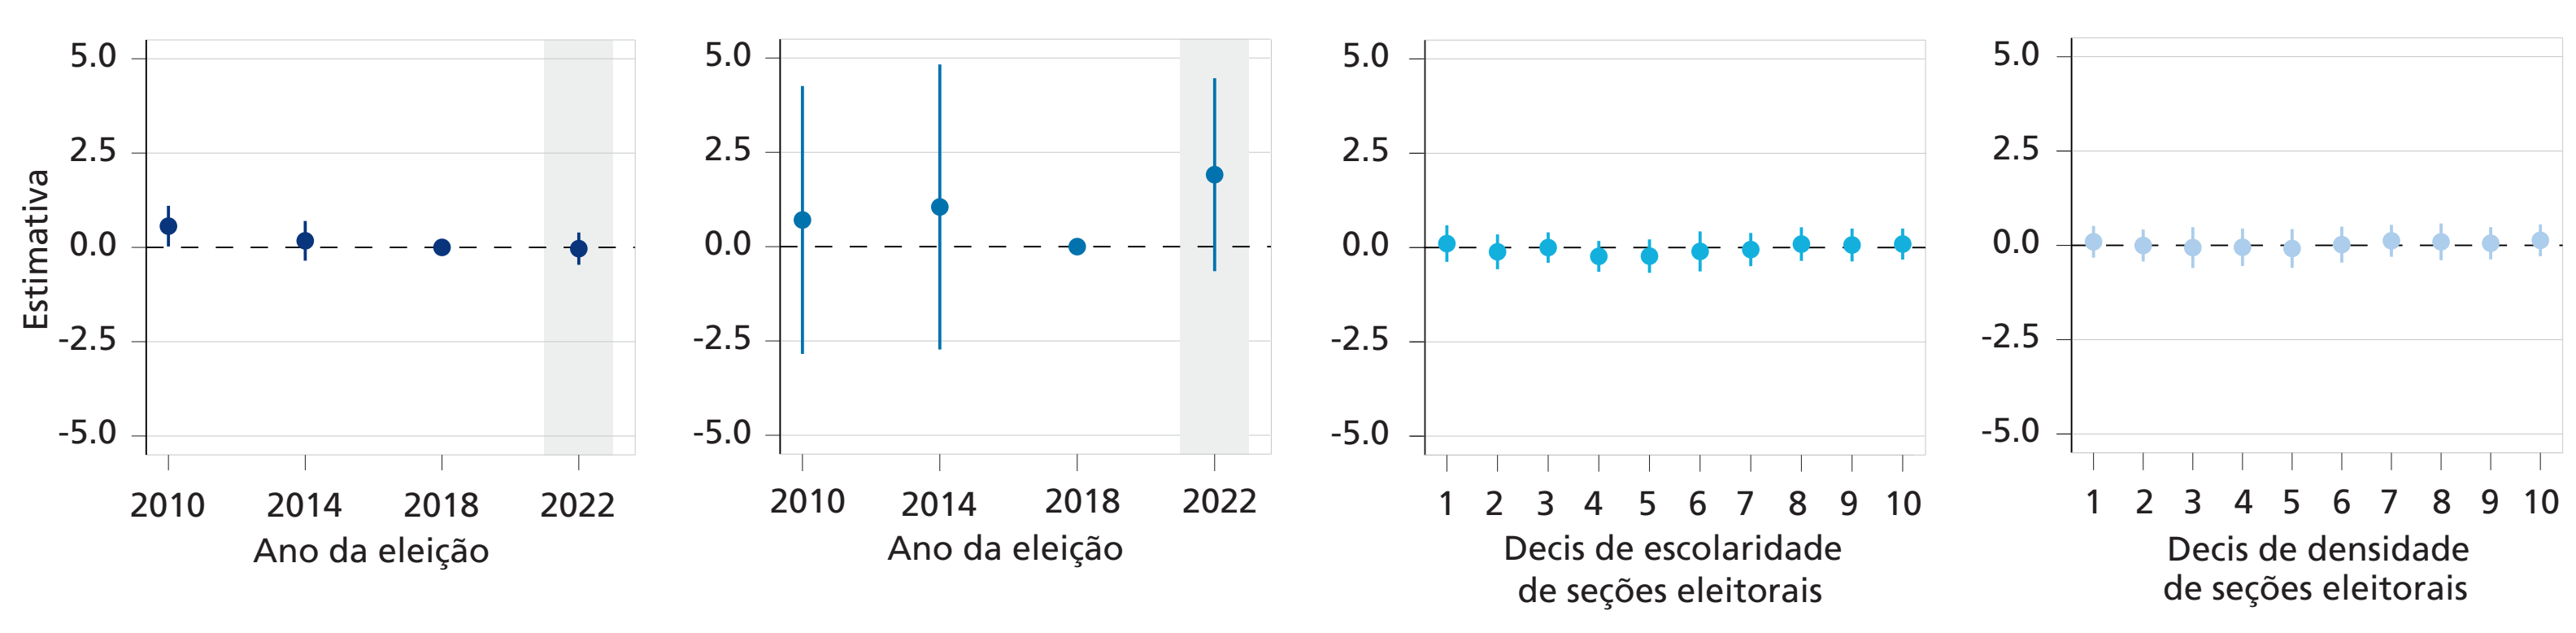
\includegraphics[width = \linewidth]{passe-livre/graficos/pereira_abst.png}
    \caption{Efeitos da política de passe livre no transporte público sobre: comparecimento eleitoral
(A), parcela de votos para o PT (B), comparecimento em seções eleitorais com diferentes
níveis socioeconômicos (C) e comparecimento em seções eleitorais em áreas com menor
e maior densidade populacional (D)}
    \subcaption*{Fonte: \cite{pereira2023transporte}}
    \label{fig_pereira_abst}
\end{figure}

Em relação a conclusão do artigo de que não houve efeito do passe livre na abstenção, novamente faltou uma discussão dos autores sobre a hipótese de identificação. No gráfico \ref{fig_pereira_abst}A, os pesquisadores medem se nos grupos de tratamento há um aumento na diferença de comparecimento do segundo e primeiro turnos em relação ao grupo de controle. Todavia, há apenas as eleições de 2010 e 2014 para fazer testes de robustez e é identificado um efeito placebo em 2010. Dessa forma, a interpretação dos resultados deveria ser que não foi possível medir o efeito do passe livre, ao invés da interpretação feita de que não houve efeito. Em outras palavras, um efeito inconclusivo é diferente de não haver efeito.

No gráfico \ref{fig_pereira_abst}C os autores fizeram uma análise de efeito heterogêneo com base em diferentes ``níveis socioeconômicos''. Entretanto, utilizaram a medida de anos de educação disponibilizada pelo TSE para separar os grupos, que é completamente defasada, visto que é apenas atualizada quando o eleitor atualiza seu título, um evento raro. Ainda sobre níveis socioeconômicos, os autores utilizam como variável de controle o PIB per capita ao longo dos anos, mas essa medida não foi divulgada para 2022 e os autores não comentaram como lidaram com essa defasagem.

De maneira geral, afirmar que o passe livre aumentou a mobilidade, mas as pessoas ao invés de votar foram aos parques implicaria ignorar todas as limitações do modelo empírico adotado na pesquisa.

\subsection{Dados}

O passe livre foi uma medida adotada em nível municipal, então os dados foram coletados também nessa escala. Para aumentar a robustez da análise, os dados foram organizados em painel, com todas as eleições nos últimos 20 anos, desde 2002. Para fins de comparação de comparáveis, foram apenas analisadas os anos de eleições presidenciais. Algumas variáveis são diferentes para o primeiro e segundo turno, como a abstenção e passe livre, mas outras como o PIB \textit{per capita} não. Os dados foram coletados para todos os municípios brasileiros.


\begin{table}
\centering
\begin{tabular}[t]{llrrrrrr}
\toprule
\multicolumn{2}{c}{ } & \multicolumn{3}{c}{Primeiro Turno} & \multicolumn{3}{c}{Segundo Turno} \\
\cmidrule(l{3pt}r{3pt}){3-5} \cmidrule(l{3pt}r{3pt}){6-8}
  & Passe Livre & Mean & SD & N & Mean & SD & N\\
\midrule
Abstenção & Não Houve & \num{0.21} & \num{0.05} & 5437 & \num{0.21} & \num{0.05} & 5148\\
 & Houve & \num{0.20} & \num{0.03} & 81 & \num{0.20} & \num{0.03} & 370\\
\bottomrule
\end{tabular}
\caption{Abstenção e tamanho amostral para cada grupo em 2022}
\label{tab_descritiva}
\end{table}

\textcite{smets2013embarrassment} conduziram uma meta análise de 90 estudos empíricos que foram publicados nos jornais de maior renome durante a década de 2000 que estudaram a abstenção de votos. Como variáveis a nível individual que foram consideradas relevantes, estão a idade, escolaridade e renda. Os dados do TSE são segmentados por faixa etária, gênero e escolaridade, mas o dado da escolaridade não é de qualidade, visto que não é atualizado regularmente - apenas quando há uma atualização do título de eleitor. Para contornar este problema, seria ideal analisar pela PNAD a média de anos de estudo na população, mas dessa forma não haveria cobertura de todos os municípios do Brasil. A \textit{proxy} adotada foi a nota do IDEB do município, um índice de educação básica calculado com base no Censo Escolar e desempenho no Sistema de Avaliação da Educação Básica (Saeb). Quanto aos dados de renda, os dados de PIB \textit{per capita} a nível municipal foram coletados do IBGE.

Para fazer o balanceamento dos grupos, foram utilizadas algumas variáveis do censo de 2010. Apesar do censo estar bastante desatualizado, as variáveis se referem a fatores estruturais dos municípios, que não mudam muito ao longo do tempo, então o viés não é muito significativo.

Em relação às variáveis do modelo microeconômico, nem todos os componentes são observáveis. O $\alpha$ e $B_s$, por exemplo, são extremamente subjetivos, o que os torna praticamente imensuráveis. A literatura identificou alguns fatores que podem contribuir com o dever cívico do voto, $D$, como a participação da população em organizações políticas, filiação partidária, número de funcionários públicos, etc. A maioria desses fatores são invariantes no tempo e são relacionados à cultura do município. Uma variável de controle adotada foi a participação do governo no PIB municipal, também obtida através do IBGE. 

Em relação ao custo de votar, muitos componentes estão envolvidos. Entre eles, o custo do transporte, a distância às urnas, demora e filas, chuvas fortes, etc. Pela dificuldade de mensurar esses fatores, foi adotada apenas uma variável mensurável, que é o número de eleitores por urna - pode indicar se há grandes filas. Foram coletados os dados históricos pluviométricos disponibilizados pelo INMET para identificar se choveu no dia da eleição, mas há muitos dados faltantes, o que pode prejudicar a análise, inviabilizando a utilização desses dados. Já os componentes $K, E, N, t$ são obtidos ou calculados através dos dados do TSE e IBGE.

A descrição mais detalhada das variáveis adotadas se encontra na tabela \ref{tab_variaveis}.

\begin{table}
    \centering
    \begin{tabular}{m{0.18\linewidth}|m{0.7\linewidth}}
        Variável & Descrição \\
        \toprule
        Tratamento & Variável binária que assume 1 caso o município tenha recebido passe livre e 0 caso contrário \\
        \midrule
        Competitividade & Quão proximos foram os resultados entre primeiro e segundo candidatos. Calculado por $1/[\log({V_A/V_B})]$, na qual $V_A$ representa o número de votos recebidos pelo candidato mais votado e $V_B$, pelo segundo candidato mais votado. \\
        \midrule
        População & População do município \\
        \midrule
        PIB per capita & PIB per capita do municipio, disponível até 2020. Para 2022, foram utilizados os últimos dados disponíveis, de 2020. \\
        \midrule
        Beneficiados & Número de pessoas no municipio dividido pela quantidade de eleitores aptos. \\
        \midrule
        IDEB & Nota da educacao dos anos finais do ensino fundamental nas escolas publicas. A nota é apenas calculadas nos anos ímpares, com o primeiro dado disponível em 2005, então foram utilizados dados defasados em um ano. \\
        \midrule
        PIB governo & É definido como valor adicionado bruto a preços correntes da administração, defesa, educação e saúde públicas e seguridade social dividido pelo PIB municipal. \\
        \midrule
        Eleitores por seção & Média do número de eleitores aptos por seção eleitoral no município

    \end{tabular}

    \caption{Variáveis utilizadas nos modelos econométricos}
    \label{tab_variaveis}
\end{table}

% \begin{table}
%     \centering
%     \begin{tabular}[t]{llrrrrrr}
%     \toprule
%     \multicolumn{2}{c}{ } & \multicolumn{3}{c}{Primeiro Turno} & \multicolumn{3}{c}{Segundo Turno} \\
%     \cmidrule(l{3pt}r{3pt}){3-5} \cmidrule(l{3pt}r{3pt}){6-8}
%       & Passe Livre & Mean & SD & N & Mean & SD & N\\
%     \midrule
%     Abstenção & Não Houve & \num{0.21} & \num{0.05} & 5437 & \num{0.21} & \num{0.05} & 5148\\
%      & Houve & \num{0.20} & \num{0.03} & 81 & \num{0.20} & \num{0.03} & 370\\
%     \bottomrule
%     \end{tabular}
%     \caption{Abstenção e tamanho amostral para cada grupo em 2022}
%     \label{tab_descritiva}
%     \end{table}

\subsection{Metodologia}

A estratégia adotada foi de realizar um \textit{diff-in-diff} com efeitos fixos de tempo e município no qual o grupo de tratamento é composto pelos municípios que adotaram o passe livre e o de controle, pelos que não adotaram. A hipótese de identificação é de que os grupos apresentam trajetórias de abstenção paralelas ao longo das eleições e, portanto, caso a diferença entre os grupos mude apenas no ano de tratamento, isso é consequência do tratamento.

\begin{equation}
\label{eq_econometric}
    \log{(y_{it})}=\beta\text{Passe Livre}_{it} + X_{it}\gamma + \alpha_t + \delta_i + \epsilon_{it}
\end{equation}

Na equação \ref{eq_econometric}, $y_{ti}$ representa a abstenção no ano $t$ para o município $i$ e $X_{it}$ representa um vetor de covariantes. O coeficiente $\beta$ captura o efeito médio do passe livre no $\log$ da abstenção e $\alpha_t$ e $\delta_i$ representam os efeitos fixos de tempo e município, respectivamente. A variável Passe Livre assume o valor 1 em 2022 para os municípios que adotaram o passe livre, caso contrário, assume zero. As estimações foram feitas separadamente para o primeiro e segundo turnos. 

A variável passe livre é endógena, já que não foi decidido de forma aleatória qual município adotaria o passe livre. Portanto, a hipótese de identificação não se sustenta, pois os grupos de controle e tratamento são muito diferentes e não podem ser comparados diretamente. Para lidar com essa questão, foi utilizado o método do \textit{Propensity Score Matching}, no qual calcula-se a probabilidade do passe livre ser adotado e compara-se municípios com propensões a ser tratados parecidas. O PSM foi calculado a partir do \textit{Nearest Neighbor} ou ``vizinho mais próximo'' com reposição.

Como discutido e observado na Figura \ref{fig_staticA}, mudanças no custo afetam de forma diferente municípios que apresentam diferentes faixas de abstenção. Nesse sentido, a modelagem da abstenção em termos logarítmicos lineariza essa relação, diminuindo o viés oriundo da heterogeneidade. 

\subsection{Resultados empíricos}

Considerando a endogeneidade discutida, o primeiro passo adotado foi fazer o \textit{Propensity Score Matchin}g (PSM). Na figura \ref{fig_balanceamento} é possível observar o suporte comum antes e depois de aplicar o método do PSM. O eixo $x$ dos gráficos se refere à probabilidade do município receber o tratamento, enquanto o $y$ se trata da densidade de probabilidade. Na figura \ref{fig_posPSM} identifica-se uma grande sobreposição nas probabilidades dos grupos de receber o tratamento, uma evidência de que os municípios que estão sendo comparados são muito semelhantes, menos em relação a receber o tratamento. O suporte comum é menos significativo no primeiro turno porque menos municípios foram tratados, então é mais difícil de encontrar vizinhos próximos.

\begin{figure}[!ht]
    \begin{subfigure}[t]{0.49\linewidth}
      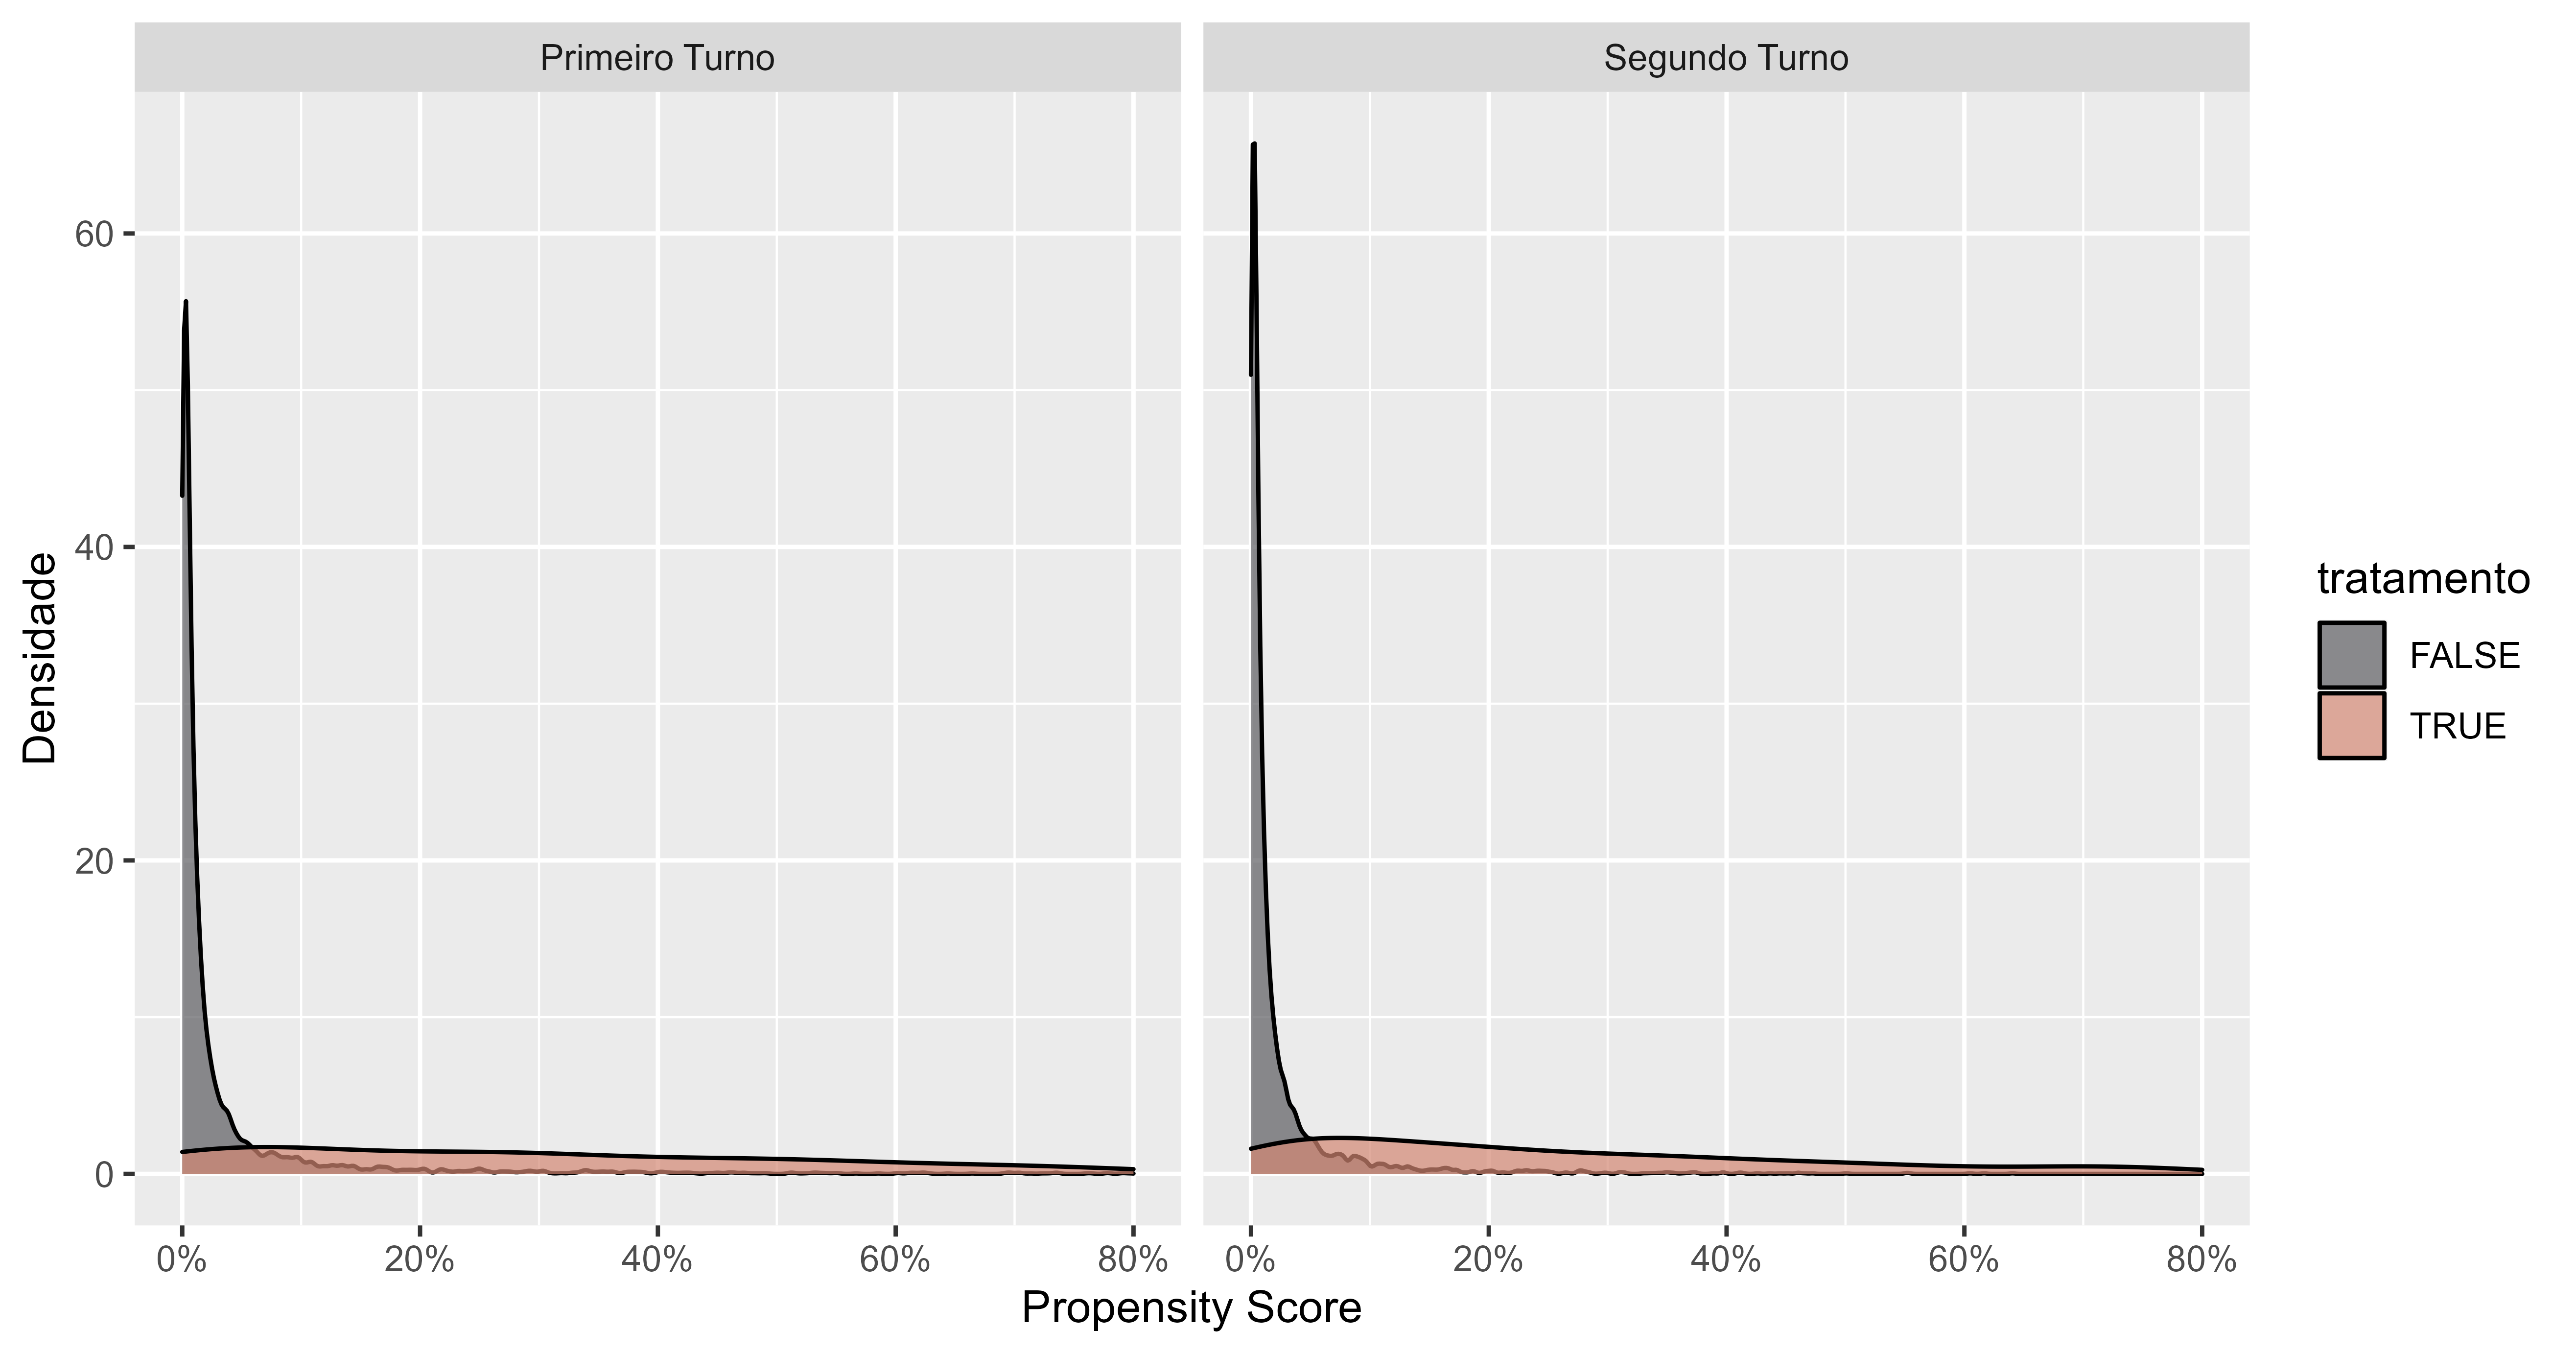
\includegraphics[width = \linewidth]{passe-livre/graficos/pre-propensity.png}
      \caption{Antes do PSM}
      \label{fig_prePSM}
    \end{subfigure}
    \hfill
    \begin{subfigure}[t]{0.49\linewidth}
      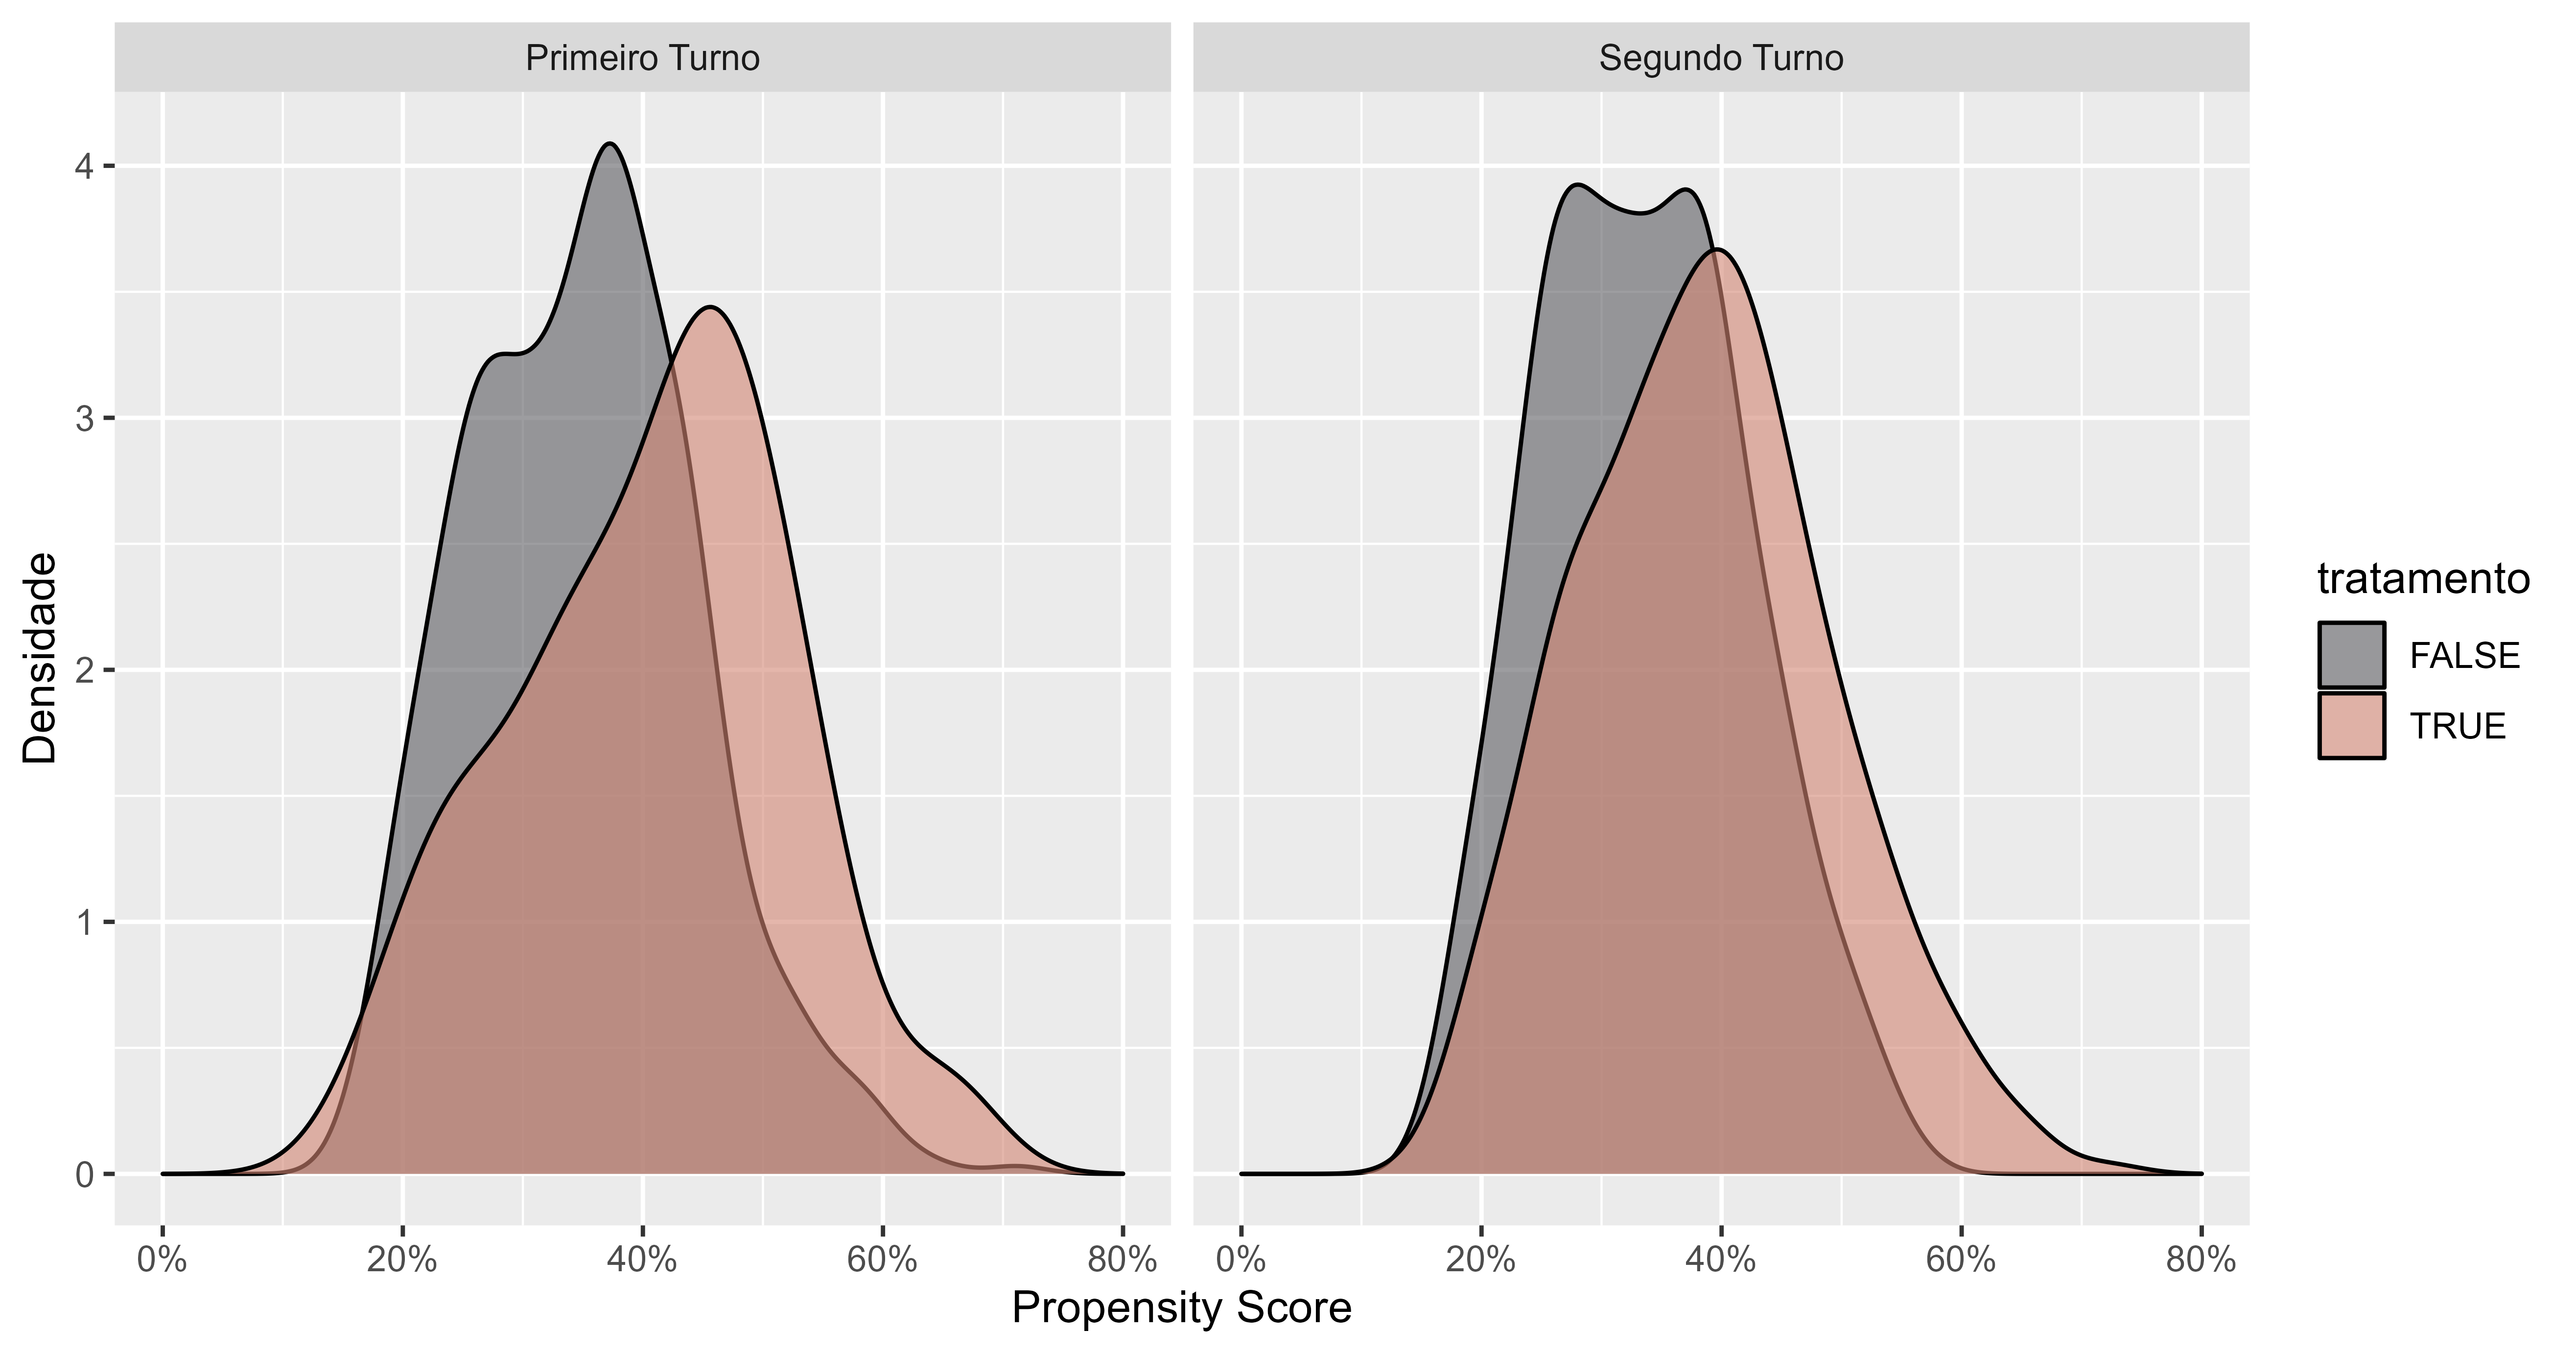
\includegraphics[width = \linewidth]{passe-livre/graficos/pos-propensity.png}
      \caption{Depois do PSM}
      \label{fig_posPSM}
    \end{subfigure}
    \caption{Balanceamento dos grupos antes e depois do \textit{Propensity Score Matching} (PSM)}
    \label{fig_balanceamento}
  \end{figure}

Depois do balanceamento dos grupos, foi conduzido um \textit{event study} (Tabela \ref{tab_eventStud}), para que se verifique a paralelidade das tendências dos diferentes grupos a partir de testes placebos. Foi escolhido como referência o ano de $t-1$, que neste caso é 2018. Caso se identifique efeito no tratamento em um ano que não teve tratamento, há uma forte evidência de que as trajetórias não são paralelas. O \textit{event study} foi conduzido com variáveis controle e sem. A descrição detalhada das variáveis se encontra na tabela \ref{tab_variaveis}.

A partir dos resultados da tabela \ref{tab_eventStud}, a hipótese de identificação não se sustenta para o primeiro turno, visto que foi observado um efeito do passe livre na abstenção em 2014, para o nível de significância de 5\%, o que é impossível, visto que não houve passe livre em 2014. Para o segundo turno não há evidências que rejeitem a hipótese de paralelismo das tendências, mas também não há evidências que apontem para um efeito do passe livre na abstenção.

\begin{table}
\centering
\begin{tabular}[t]{lcccc}
\toprule
& \multicolumn{2}{c}{Sem Controles} & \multicolumn{2}{c}{Com Controles} \\
  \cmidrule(lr){2-3} \cmidrule(lr){4-5}
  & Primeiro Turno & Segundo Turno & Primeiro Turno & Segundo Turno\\
\midrule
tratamento:2002 & \num{-0.069} (\num{0.290}) & \num{0.044} (\num{0.216}) &  & \\
tratamento:2006 & \num{-0.044} (\num{0.379}) & \num{0.024} (\num{0.451}) & \num{-0.049} (\num{0.273}) & \num{0.027} (\num{0.238})\\
tratamento:2010 & \num{-0.068} (\num{0.196}) & \num{0.003} (\num{0.904}) & \num{-0.069} (\num{0.109}) & \num{0.008} (\num{0.681})\\
tratamento:2014 & \num{-0.146} (\num{0.005}) * & \num{-0.010} (\num{0.627}) & \num{-0.090} (\num{0.023}) * & \num{-0.001} (\num{0.956})\\
tratamento:2022 & \num{-0.010} (\num{0.692}) & \num{0.016} (\num{0.182}) & \num{-0.026} (\num{0.282}) & \num{0.003} (\num{0.803})\\
log(Competitividade) &  &  & \num{-0.024} (\num{<0.001}) * & \num{-0.010} (\num{0.018}) *\\
log(PIB per capita) &  &  & \num{-0.022} (\num{0.043}) * & \num{-0.016} (\num{<0.001}) *\\
log(Beneficiados) &  &  & \num{-0.865} (\num{<0.001}) * & \num{-0.857} (\num{<0.001}) *\\
IDEB &  &  & \num{-0.063} (\num{0.002}) * & \num{-0.062} (\num{<0.001}) *\\
log(População) &  &  & \num{0.176} (\num{0.287}) & \num{0.164} (\num{0.089})\\
log(PIB governo) &  &  & \num{-0.018} (\num{0.005}) * & \num{-0.011} (\num{<0.001}) *\\
log(Eleitores por seção) &  &  & \num{0.711} (\num{<0.001}) * & \num{0.298} (\num{<0.001}) *\\
\midrule
Num.Obs. & \num{972} & \num{4440} & \num{802} & \num{3656}\\
R2 & \num{0.567} & \num{0.590} & \num{0.706} & \num{0.709}\\
R2 Adj. & \num{0.483} & \num{0.526} & \num{0.631} & \num{0.651}\\
R2 Within & \num{0.021} & \num{0.004} & \num{0.276} & \num{0.184}\\
R2 Within Adj. & \num{0.015} & \num{0.002} & \num{0.263} & \num{0.181}\\
\bottomrule
\end{tabular}
\caption{Resultado do \textit{event study} com efeito fixo de tempo e município, estimações por MQO}
\label{tab_eventStud}
\end{table}

É relevante destacar que as variáveis de controle selecionadas se mostraram bastante relevantes e apresentam o sinal esperado, o que aponta na mesma direção da literatura teórica e outros estudos empíricos. Os coeficientes do primeiro turno são semelhantes aos do segundo turno, com exceção da competitividade e eleitores por seção, que se mostram menos relevantes no segundo turno. Entretanto, a variável de interesse a partir dessa estratégia não se demonstra relevante.

Com isso, foi feita uma análise de efeito heterogêneo de renda. Como descrito com melhor detalhe na seção \ref{subsec_revisLit} e na figura \ref{fig_static2}, uma redução no custo de votar afeta de formas diferentes cada município e uma variável importante que define essa diferença é o nível de renda do município. Portanto, foram separados os municípios em 4 quantis de renda e foi conduzido novamente o \textit{event study} separadamente para cada um desses grupos (Figura \ref{fig_eventStud}). 

\begin{figure}[!ht]
    \begin{subfigure}[t]{0.49\linewidth}
      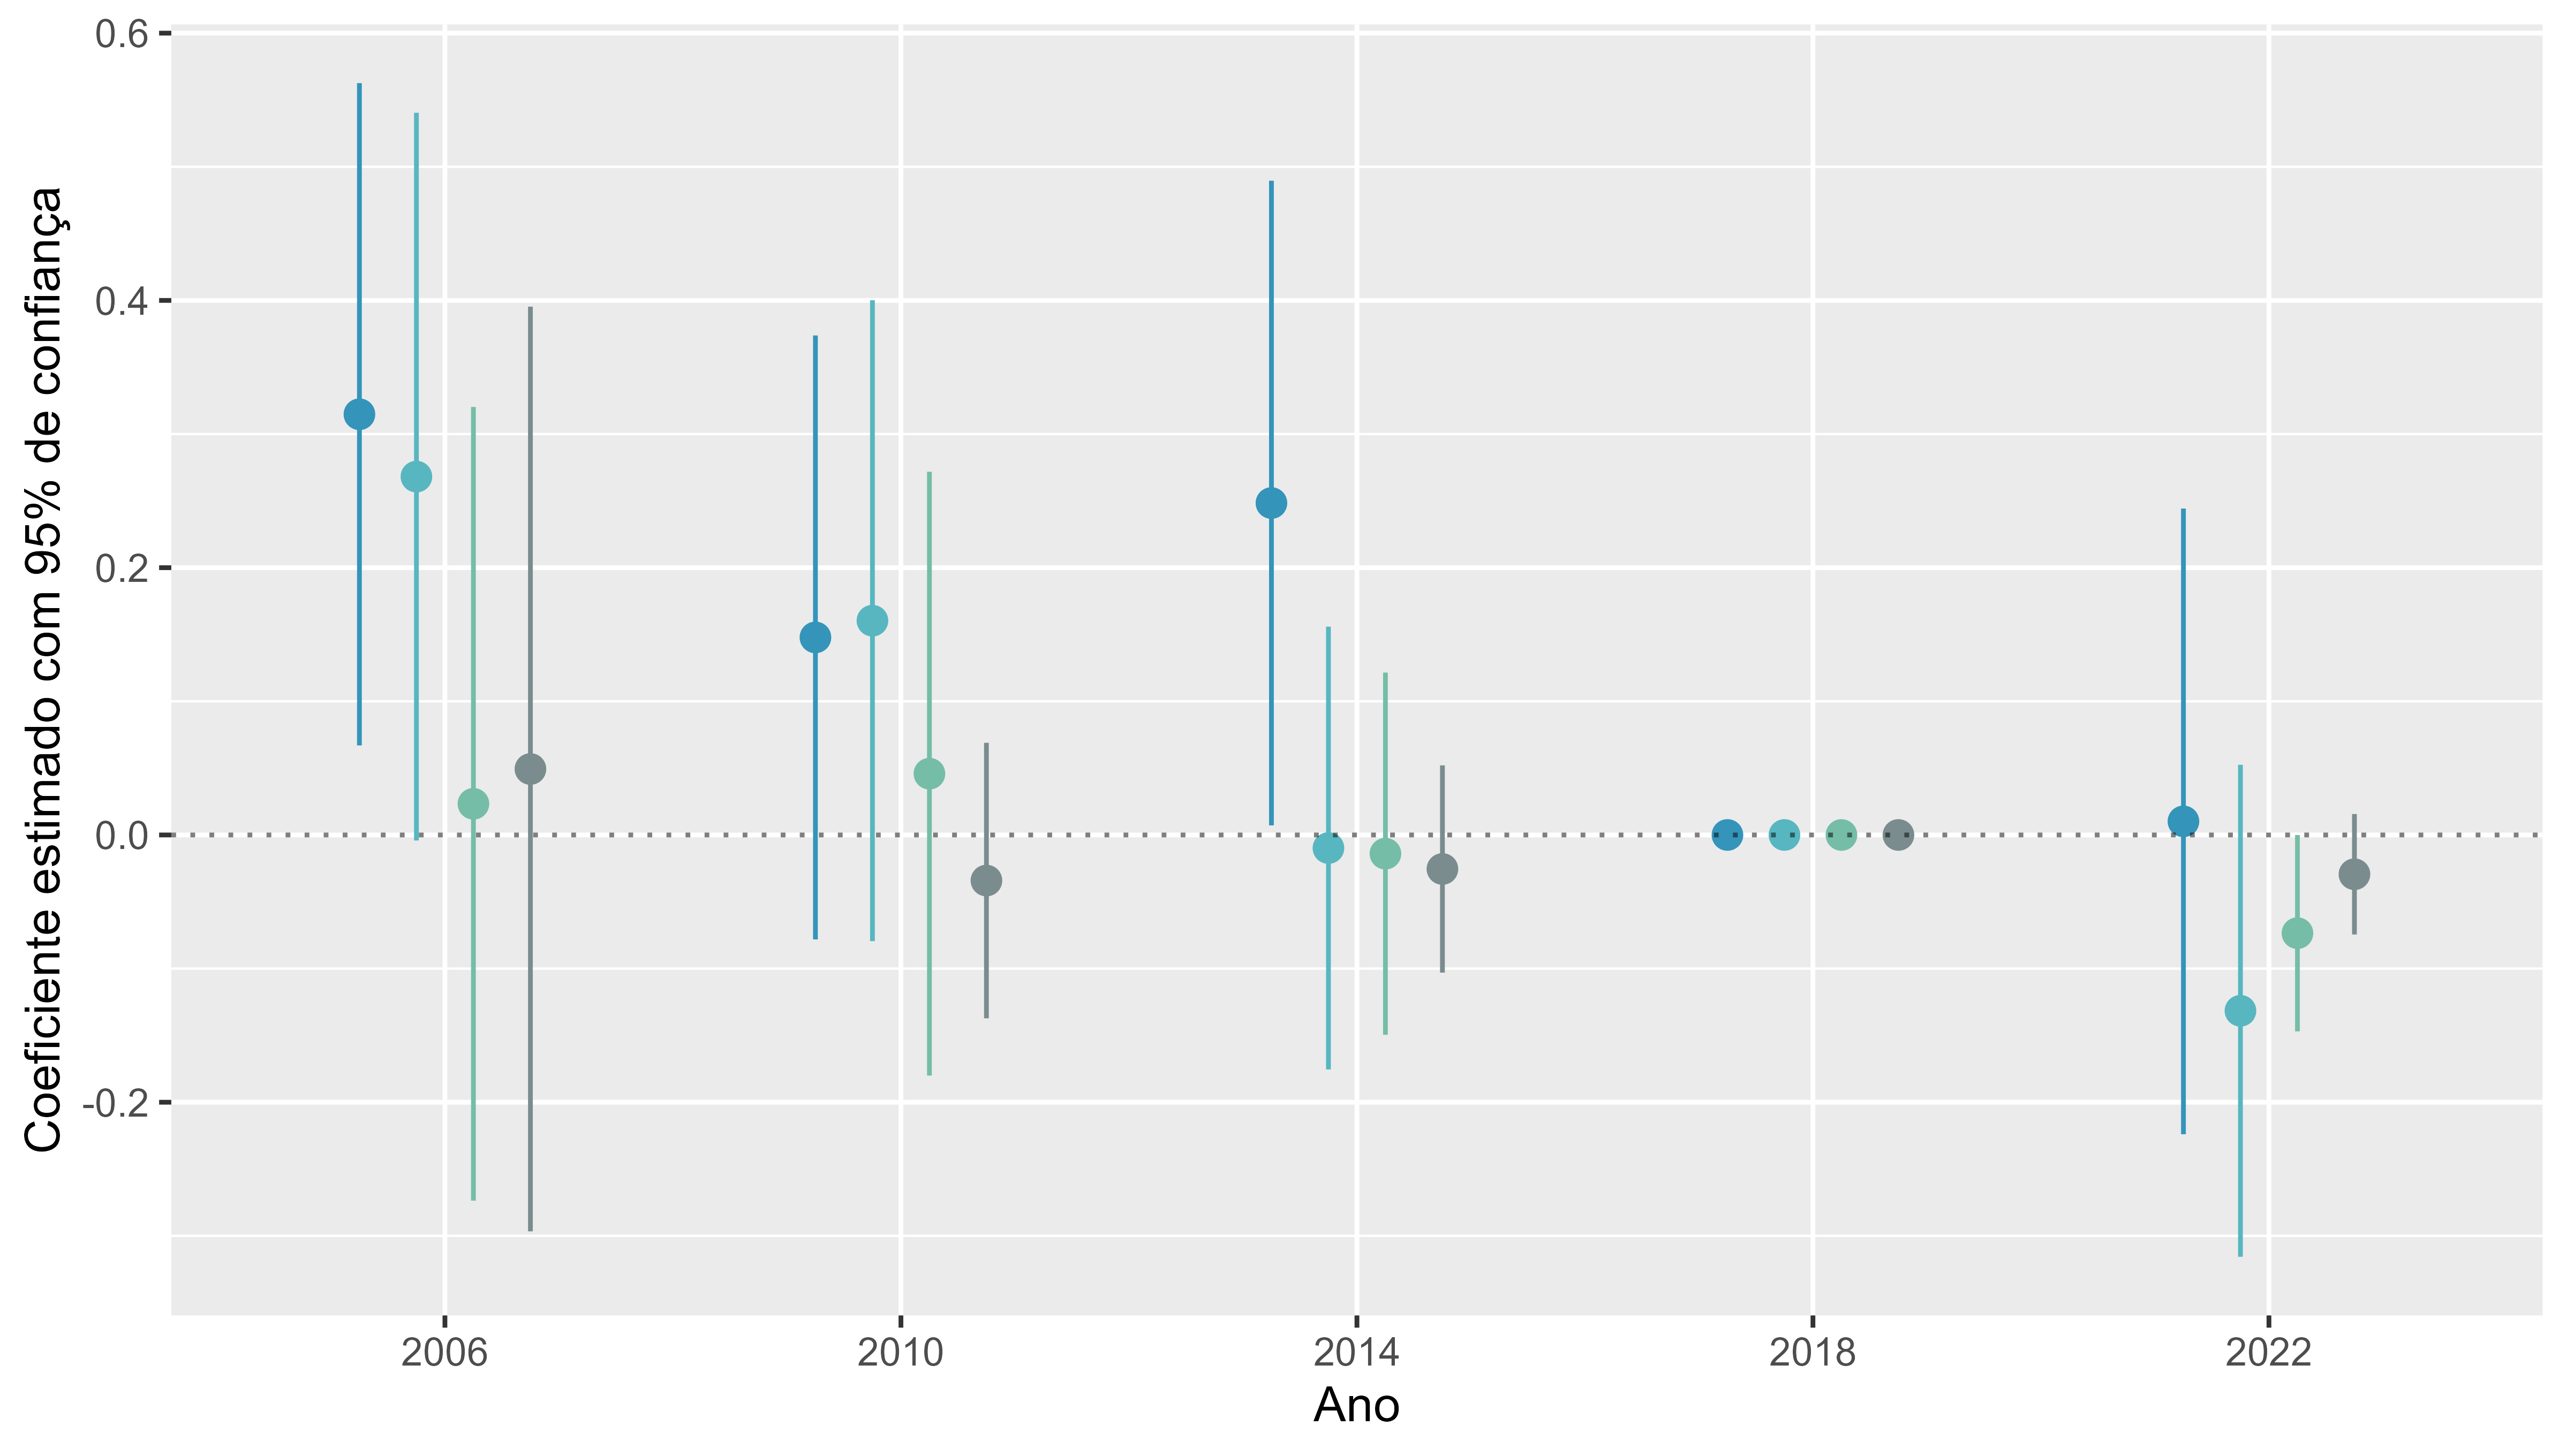
\includegraphics[width = \linewidth]{passe-livre/graficos/event_study_heter_1t.png}
      \caption{Primeiro Turno}
      \label{fig_eventStud1}
    \end{subfigure}
    \hfill
    \begin{subfigure}[t]{0.49\linewidth}
      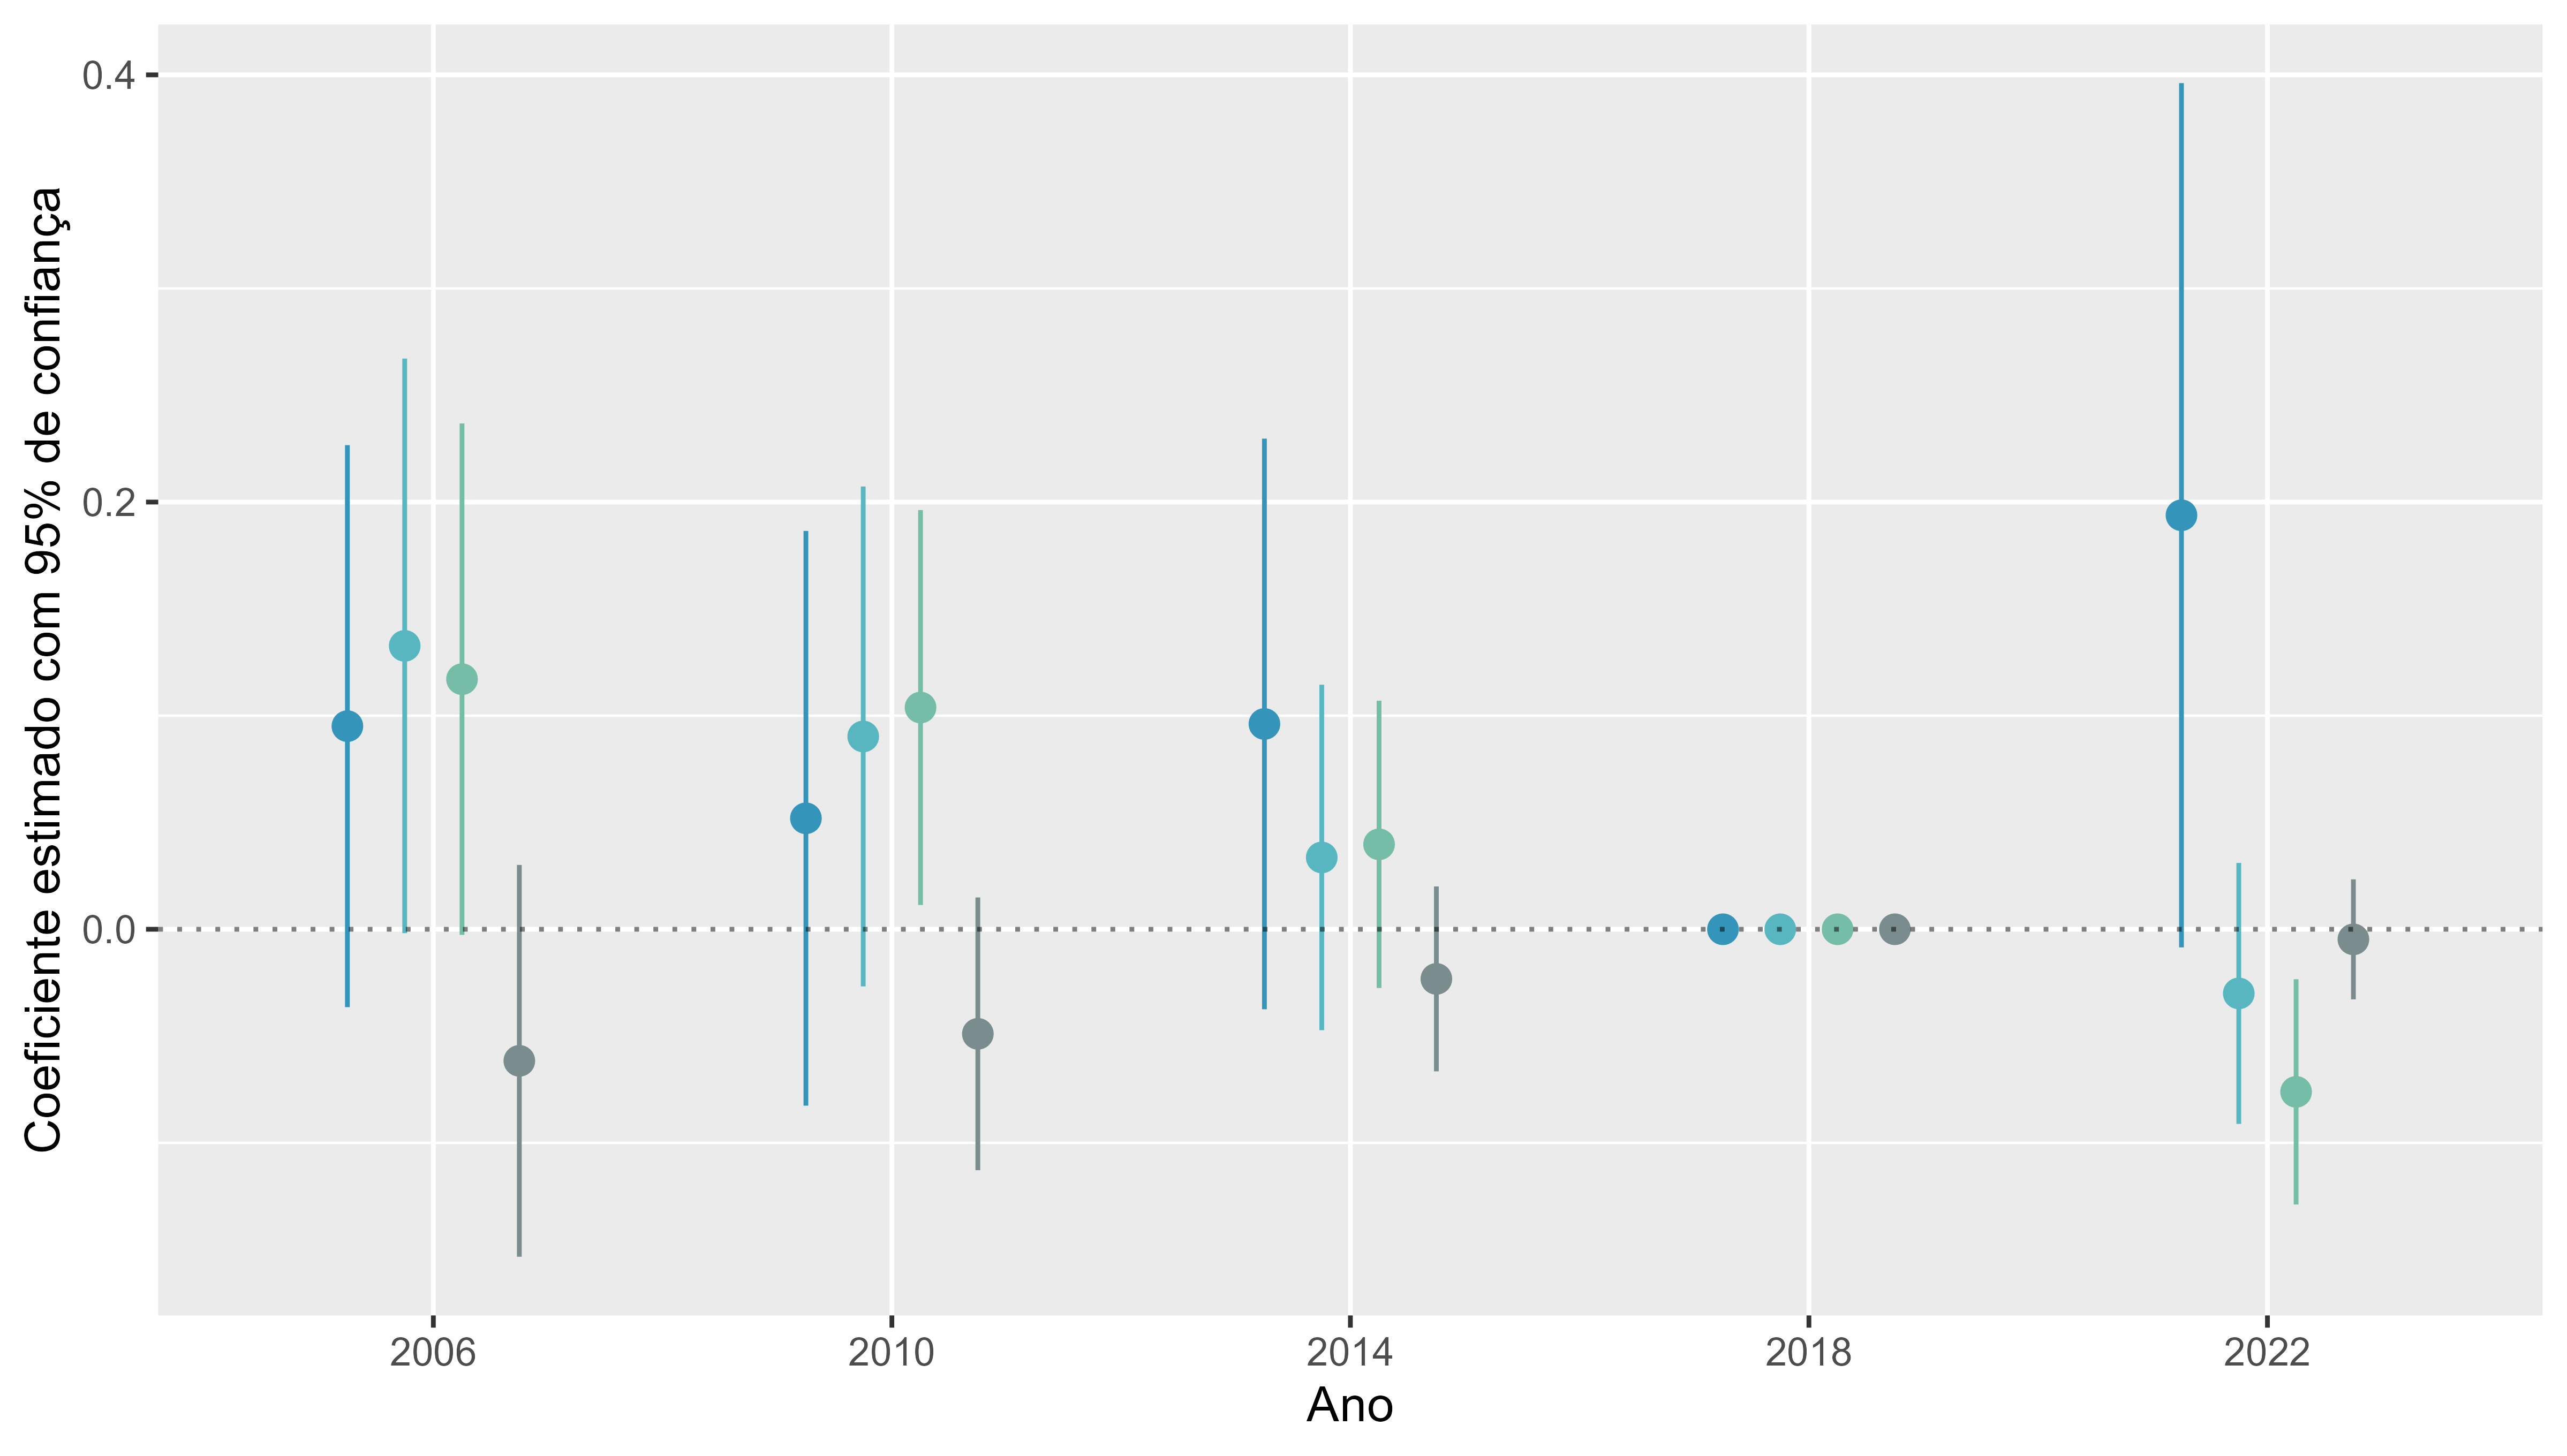
\includegraphics[width = \linewidth]{passe-livre/graficos/event_study_heter_2t.png}
      \caption{Segundo Turno}
      \label{fig_eventStud2}
    \end{subfigure}
    \caption{Análise de efeito heterogêneo através de um \textit{event study}}
    \subcaption*{O quartil à esquerda se refere ao quartil mais pobre e o da direita, o mais rico}

    \label{fig_eventStud}
  \end{figure}

A partir da análise da Figura \ref{fig_eventStud}, fica evidente a dificuldade de validar a hipótese de identificação, visto que com 95\% de confiança observa-se mais de uma vez efeito placebo em anos de eleição nas quais não houve tratamento, principalmente quando a amostra é dividida em quatro e perdem-se muitos graus de liberdade. Entretanto, para o terceiro quartil de renda foi identificada uma redução na abstenção do segundo turno com 5\% de significância. Com base nos resultados do \textit{event study} como um todo, o efeito do passe livre na abstenção é inconclusivo utilizando a estratégia empírica escolhida, dada a fragilidade da hipótese de identificação.

\subsection{Limitações}

A principal limitação do estudo empírico conduzido, como mencionado anteriormente, foi a dificuldade de validar a hipótese de identificação da metodologia escolhida. Como o intervalo de tempo de quatro anos entre as eleições é muito grande, muitos fatores em um município mudam de uma votação para outra e depois de apenas 5 eleições, já se passaram 20 anos, tornando eleições distantes praticamente incomparáveis do ponto de vista empírico. Nesse sentido, seria importante conduzir um estudo com um método que não precise comparar os resultados de 2022 com a eleição anterior.

Outra dificuldade é oriunda da endogeneidade na decisão de adotar ou não o tratamento. Mesmo depois do balanceamento dos grupos, eles se mostraram não tão comparáveis, o que indica que o perfil de município que adotou o passe livre é bastante diferente do perfil dos que não adotaram. Informações como se o município escolheu adotar o passe livre ou foi obrigado a fazê-lo podem ajudar a entender o perfil do município tratado e balancear melhor os grupos.

Além disso, há uma grande defasagem nas variáveis. O PIB \textit{per capita}, por exemplo não foi divulgado ainda para o ano de 2022, e foi necessário utilizar o dado desatualizado de 2020, o que pode gerar viés. Ademais, as variáveis utilizadas para o balanceamento, estão defasadas em 12 anos. Como já foi discutido, essa defasagem não é tão importante quanto a dos dados para a regressão principal, mas ainda merece ser destacada.

A cobertura do sistema de transporte público do município determina quantas pessoas efetivamente conseguem usufruir do benefício do passe livre e para resultados mais robustos isso teria que ser considerado. Por fim, como discutido na seção teórica, a assimetria de informação é uma variável extremamente relevante para determinar o sucesso ou fracasso do passe livre e isso não foi contabilizado ou considerado na análise empírica. 

\section{Conclusão}

Pelas limitações e dificuldades apresentadas, os resultados empíricos em relação ao efeito do passe livre na abstenção são inconclusivos. Nesse sentido, o único resultado que pode ser validado é o teórico. O que a teoria microeconômica indica é que, assumindo as premissas do modelo, uma redução no custo do voto leva a um maior comparecimento quando não há assimetria de informação, mesmo que muito pequeno. Entretanto, não há evidências de que o passe livre foi adotado de maneira eficiente \footnote{Eficiente se refere à uma maneira que todos os habitantes estão cientes da medida e que ela não gere assimetria de informação. Neste caso, os eleitores antecipariam de maneira correta a quantidade de pessoas que seriam ``convencidas'' a votar, mesmo que seja apenas 1 pessoa}, então pode ser que a medida realmente não tenha apresentado efeito de reduzir a abstenção em 2022.

Por outro lado, o que a teoria indica é que se um município adotar o passe livre de maneira eficiente, a abstenção será reduzida. Na medida em que a adoção é mais ineficiente, têm-se um \textit{moral hazard} e, como discutido na figura \ref{fig_static4}, o efeito do passe livre pode ser atenuado ou pode até acabar sendo o efeito contrário em um caso extremo. 

Nesse sentido, caso seja adotada a medida, há alguns pontos importantes para serem levados em conta. Primeiramente, é muito importante garantir que os canais de comunicação do governo trabalhem de forma a fazer a notícia chegar em todos, principalmente aqueles que usufruem do sistema de transporte público. Em segundo, no dia da eleição a capacidade e qualidade do transporte entregues devem ser igual ou melhor do que o prometido, para evitar que aconteça o \textit{moral hazard}.